\documentclass[tikz,border=7pt]{standalone}
\usepackage[utf8]{inputenc}
\usepackage[OT4,plmath]{polski}
\begin{document}
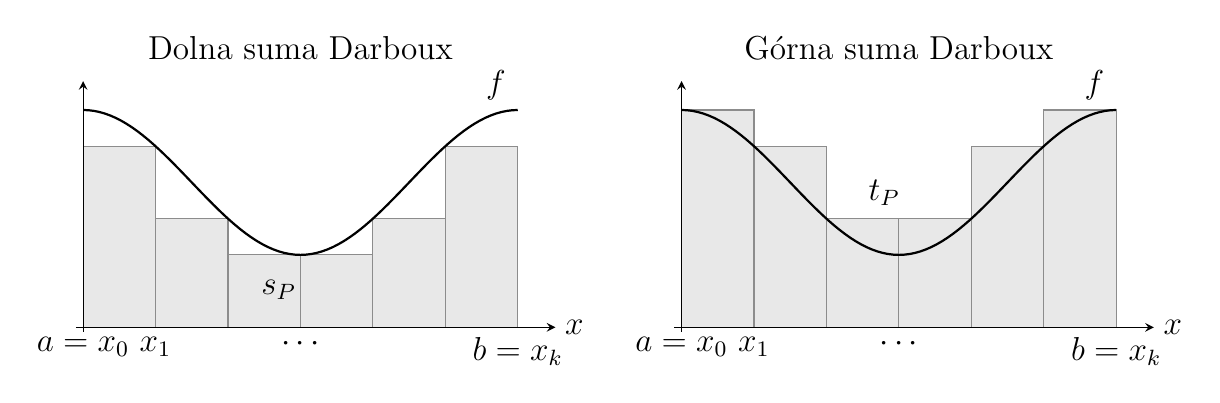
\begin{tikzpicture}[x=0.92cm,y=0.92cm,>=stealth,font=\large]
  \begin{scope}
    \node at (3,3.85) {Dolna suma Darboux};
    \foreach \i/\height in {0/2.5,1/1.5,2/1,3/1,4/1.5,5/2.5} {
      \filldraw[fill=black!9,draw=black!45]
        (\i,0) rectangle ({\i+1},\height);
    }
    \draw[thick] plot[domain=0:6,samples=81] (\x,{2+cos(60*\x)});
    \draw[->,thin] (-0.1,0) -- (6.52,0) node[right] {$x$};
    \draw[->,thin] (0,-0.06) -- (0,3.4);
    \node[above] at (5.7,3.0) {$f$};
    \node at (2.7,0.52) {$s_P$};
    \node[below] at (0,0) {$a=x_0$};
    \node[below] at (1,0) {$x_1$};
    \node[below] at (3,0) {$\cdots$};
    \node[below] at (6,0) {$b=x_k$};
  \end{scope}
  \begin{scope}[xshift=7.6cm]
    \node at (3,3.85) {Górna suma Darboux};
    \foreach \i/\height in {0/3,1/2.5,2/1.5,3/1.5,4/2.5,5/3} {
      \filldraw[fill=black!9,draw=black!45]
        (\i,0) rectangle ({\i+1},\height);
    }
    \draw[thick] plot[domain=0:6,samples=81] (\x,{2+cos(60*\x)});
    \draw[->,thin] (-0.1,0) -- (6.52,0) node[right] {$x$};
    \draw[->,thin] (0,-0.06) -- (0,3.4);
    \node[above] at (5.7,3.0) {$f$};
    \node[above] at (2.8,1.55) {$t_P$};
    \node[below] at (0,0) {$a=x_0$};
    \node[below] at (1,0) {$x_1$};
    \node[below] at (3,0) {$\cdots$};
    \node[below] at (6,0) {$b=x_k$};
  \end{scope}
\end{tikzpicture}
\end{document}
